\chapter{Selection problem}
\label{tree:S}

The selection problem is depicted as follows,

Find the element at position $k$ in a permutation of array $A$ that respects the following constraints,

\begin{equation}
\forall_{i = 0}^{i < k} \text{comp}(A_i, A_k)
\end{equation}

\begin{equation}
\forall_{i = k + 1}^{i < |A| - 1} \neg\text{comp}(A_i, A_k)
\end{equation}

where the comparison operator is usually $\leq$.\\


\begin{figure}
	\centering
	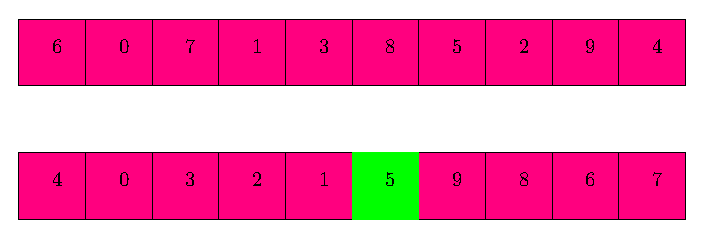
\includegraphics[width=0.5\textwidth]{fig/selection:array}
	\caption{\label{fig:selection:array} An array of 10 elements and its selection result.}
\end{figure}


\begin{theorem}
The ITLB for the selection problem is $n$.
\end{theorem}

\begin{proof}
Consider the comparison tree of the sorting problem.
Such a tree has $n!$ leafs, each leaf representing one of the permutations of $A$.
Suppose the tree is balanced.
Each time we compare 2 elements $a$ and $b$ we can discard half of the leafs since there are half of the permutations that don't respect the constraint $\text{comp}(a, b)$.
Hence the height of the comparison tree is $\log(n!) \sim n \log(n)$.

We do not need to reach a leaf to solve the selection problem.
There are in fact $(n-k)!k!$ permutations that respect the selection constraints.
Hence the length of a path in the comparison tree is now $\log(\frac{n!}{\frac{n}{2}!^2})$
for the worst case ($k = \frac{n}{2}$).

\begin{align*}
\log(\frac{n!}{\frac{n}{2}!^2})	&= \log n! - 2 \log \frac{n}{2}! \\
								&= n \log n - 2\frac{n}{2} \log \frac{n}{2} \\
								&= n \log n - n \log \frac{n}{2} \\
								&= n(\log n - \log \frac{n}{2}) \\
								&= n(\log n - \log n + \log 2) \\
								&= n
\end{align*}
\end{proof}

The Hasse diagrams for this problem are those in \ref{fig:selection:diag}.

\begin{figure}
	\centering
	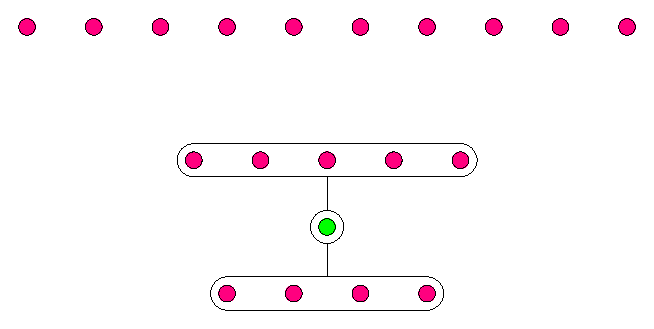
\includegraphics[width=0.6\textwidth]{fig/selection:diag}
	\caption{\label{fig:selection:diag} Hasse diagrams for the selection problem.}
\end{figure}


We have seen in this course that a randomized algorithm to solve this problem, \defineconcept{Quickselect}, has an average complexity of $3.39n$ for the median selection.